\documentclass[10pt]{article}

% Manage page layout
\usepackage[margin=2.5cm, includefoot, footskip=30pt]{geometry}
\pagestyle{plain}
\setlength{\parindent}{0em}
\setlength{\parskip}{1em}
\renewcommand{\baselinestretch}{1}

%%%%%%%PACKAGES HERE%%%%%%%
\usepackage{tikz}
\usepackage{amsmath}
\usepackage{amssymb}
\usepackage{amsthm}
\usepackage{graphicx}
\usepackage{subcaption}
\usepackage{standalone}
\usepackage{booktabs}
\usepackage{algorithm, setspace}
\usepackage[noend]{algpseudocode}

\makeatletter
\def\BState{\State\hskip-\ALG@thistlm}
\makeatother

\newcommand{\R}{\mathbb{R}}
\newtheorem{theorem}{Theorem}
\usetikzlibrary{decorations.pathmorphing, decorations.pathreplacing, angles,
                quotes, calc, er, positioning}

\newtheorem{lemma}[theorem]{Lemma}
\def\arraystretch{1.5}
%%%%%%%%%%%%%%%%%%%%%%%%%%%
\title{Stability of defection, optimisation pf strategy and the limits of memory in
the Prisoner's Dilemma.}
\author{Nikoleta E. Glynatsi \and Vincent Knight}
\date{}

\begin{document}

\maketitle

\begin{abstract}

In this manuscript we build upon a framework provided in 1989 to study best
responses in the well known memory one strategies of the Iterated Prisoner's
Dilemma. The aim of this work is to construct a compact way of identifying best
responses of short memory strategies and to show their limitations in multi-opponent
interactions. A number of theoretic results are presented. %TODO: Expand when we get results
\end{abstract}

\section{Introduction}\label{section:introduction}

The Prisoner's Dilemma (PD) is a two player person game used in understanding the
evolution of co-operative behaviour. Each player can choose between cooperation
(C) and defection (D). The decisions are made simultaneously and independently.
The normal form representation of the game is given by:

\begin{equation}\label{equ:pd_definition}
    S_p = \begin{pmatrix}
    R & S  \\
    T & P
    \end{pmatrix} \quad
    S_q = \begin{pmatrix}
        R & T  \\
        S & P
        \end{pmatrix}
\end{equation}

where \(S_p\) represents the utilities of the row player and \(S_q\) the utilities
of the column player. The payoffs, \((R, P, S, T)\) (the most common values used in the
literature are \((3, 1, 0, 5)\)~\cite{Axelrod1981}), are constrained by equations
(\ref{eq:pd_constrain_one}) and~(\ref{eq:pd_constrain_two}). Constraint
(\ref{eq:pd_constrain_one}) ensures that defection dominates cooperation and
constraint (\ref{eq:pd_constrain_two}) ensures that there is a dilemma; the sum of the
utilities for both players is better when both choose to cooperate.

\begin{equation}\label{eq:pd_constrain_one}
    T > R > P > S 
\end{equation}

\begin{equation}\label{eq:pd_constrain_two}
    2R > T + S
\end{equation}

The PD is a one shot game, however it is commonly studied in a manner where the
history of the interactions matter. The repeated form of the game is called the
Iterated Prisoner's Dilemma (IPD) and in the 1980s following the work of
\cite{Axelrod1980a, Axelrod1980b} it attracted the attention of the scientific
community.

In~\cite{Axelrod1980a} and~\cite{Axelrod1980b}, the first well known computer
tournaments of the IPD were performed. A total of 13 and 63 strategies were submitted
in computer code and competed against each other in a round robin tournament.
All contestants competed against each other, a copy of themselves and a random strategy.
The winner was decided on the average score a strategy achieved and not the total number
of wins. How many turns of history that a strategy would use, the memory size, was left
to the creator of the strategy to decide.

The winning strategy of both tournaments was a strategy called Tit for Tat. Tit for Tat
is a strategy which starts by cooperating and then mimics the last move of
it's opponent. This is a strategy which makes use of the previous move of the opponent
only and a reactive strategy. In~\cite{Nowak1989} a framework for
studying such strategies was introduced. This was later used to introduce well known
reactive strategies such as Generous Tit For Tat~\cite{Nowak1990}.

Reactive strategies are a subset of memory one strategies. Memory one strategies
similarly are only concerned with the previous turn. However, they take into consideration
both players' recent moves to decide on an action. Several successful memory one
strategies are found in the literature, for example Pavlov~\cite{Nowak1993}.

A well known set of memory on strategies was introduced in~\cite{Press2012},
these were called zero determinant (ZD) strategies. The ZD strategies manage to force a linear
relationship between the score of the strategy and the opponent. According to~\cite{Press2012}
the ZD strategies can dominate any evolutionary opponent in pairwise
interactions by using a single slot of memory. Thus the usefulness of memory in
the IPD was questioned.

The ZD strategies attracted a lot of attention. It was stated that
``Press and Dyson have fundamentally changed the viewpoint on the Prisoner's
Dilemma''~\cite{Stewart2012}. In~\cite{Stewart2012} a very similar tournament to Axelrod's
tournament is run including ZD strategies and a new set of ZD strategies the Generous
ZD. One specific advantage of memory one strategies is their mathematical tractability.
As described in Section~\ref{section:utility_against_mem_one}
they can be represented completely as an element of \(\R^{4}\).

Even so, ZD and memory one strategies have also received criticism. In~\cite{Harper2015},
the `memory of a strategy does not matter' statement was questioned. A set of more
complex strategies, strategies that take in account the entire history set of the
game, were trained and proven to be more robust against multiple opponents.

The purpose of this work is to consider a given memory one strategy 
in a similar fashion to~\cite{Press2012}. However whilst~\cite{Press2012} found
a way for a player to manipulate a given opponent, this work will consider a multidimensional
optimisation approach to identify the best response to a group of opponents. In
essence the aim is to produce a compact method of identifying the best memory one
strategy against a given opponent.

In the second part of this manuscript we explore the limitation of these best response
strategies. This is achieved by comparing the performance of an optimal
memory one strategy, for a given environment, with the performance of a more complex
strategy that has a larger memory.

One particular benefit of this analysis is the identification of conditions for
which defection is a best response. Thus, identifying environments for which
cooperation can not occur.

\section{The utility against memory one players}\label{section:utility_against_mem_one}

In~\cite{Press2012} a framework is described to sufficient study the interactions
of memory one strategies modelled as a stochastic process. In this manuscript it
is stated that if a strategy is concerned with only the outcome of a single turn
then there are four possible `states' the strategy could be in. These are
\(CC, CD, DC,CC\). A memory one strategy is denoted by the probabilities of
cooperating after each of these states, \(p=(p_1, p_2, p_3, p_4) \in \R_{[0,1]} ^ 4\).
A diagrammatic representation of such strategy is given in Figure~\ref{fig:diagram_mem_one}.

\begin{figure}
    \centering
    \begin{subfigure}{0.45\textwidth}
        \centering
        \includestandalone[width=.65\textwidth]{tex/states}
        \subcaption{Diagrammatic representation of a memory one strategy.}
        \label{fig:diagram_mem_one}
    \end{subfigure}
    \begin{subfigure}{0.45\textwidth}
        \centering
        \includestandalone[width=.88\textwidth]{tex/markov_chain}
        \subcaption{Markov chain on a PD game.}
        \label{fig:markov_chain}
    \end{subfigure}
\end{figure}

Moreover, if two players are moving from state to state following a general
memory one strategy this can be modelled as a Markov process. A diagrammatic
representation of the Markov chain is shown in Figure~\ref{fig:markov_chain}.
The corresponding transition matrix \(M\) given by:

\begin{equation}\label{eq:m_matrix}
    M = \left[\begin{matrix}p_{1} q_{1} & p_{1} \left(- q_{1} + 1\right) & q_{1} \left(- p_{1} + 1\right) & \left(- p_{1} + 1\right) \left(- q_{1} + 1\right)\\p_{2} q_{3} & p_{2} \left(- q_{3} + 1\right) & q_{3} \left(- p_{2} + 1\right) & \left(- p_{2} + 1\right) \left(- q_{3} + 1\right)\\p_{3} q_{2} & p_{3} \left(- q_{2} + 1\right) & q_{2} \left(- p_{3} + 1\right) & \left(- p_{3} + 1\right) \left(- q_{2} + 1\right)\\p_{4} q_{4} & p_{4} \left(- q_{4} + 1\right) & q_{4} \left(- p_{4} + 1\right) & \left(- p_{4} + 1\right) \left(- q_{4} + 1\right)\end{matrix}\right].
\end{equation}

The long run steady state probability \(v\) is the solution to \(\bigtriangledown M = \bigtriangledown\)
(given in the Appendix). %TODO include Appendix
Combining the stationary vector \(v\) with the payoff matrices of equation~(\ref{equ:pd_definition})
allow us to retrieve the expected payoffs for each player. Thus, the utility for
player \(p\) against \(q\), denoted as \(u_q(p)\), is defined by,

\begin{equation}\label{eq:press_dyson_utility}
    u_q(p) = v \times (R, P, S, T).
\end{equation}

Here we present the first theoretical result which concerns the form of \(u_q(p)\).
That is that \(u_q(p)\) is given by a ratio of two quadratic forms~\cite{kepner2011},
as presented by Theorem~\ref{theorem:quadratic_form_u}.

\begin{theorem}\label{theorem:quadratic_form_u}
    The expected utility of a memory one strategy \(p\in\mathbb{R}_{[0,1]}^4\)
    against a memory one opponent strategy \(q\in\mathbb{R}_{[0,1]}^4\), denoted
    as \(u_q(p)\), can be written as a ratio of two quadratic forms:

    \begin{equation}\label{eq:optimisation_quadratic}
    u_q(p) = \frac{\frac{1}{2}pQp^T + cp + a}
                {\frac{1}{2}p\bar{Q}p^T + \bar{c}p + \bar{a}}, 
    \end{equation}
    where \(Q, \bar{Q}\) \(\in \R^{4\times4}\) matrices defined by the transition
    probabilities of the opponent \(q_1, q_2, q_3, q_4\) as follows:
    
    \begin{center}
    \begin{equation}
    \resizebox{0.9\linewidth}{!}{\arraycolsep=2.5pt%
    \boldmath\(
    Q = \left[\begin{matrix}0 & 5 q_{4} \left(q_{1} - q_{3}\right) & - q_{4} \left(q_{1} - q_{2}\right) & \left(q_{1} - q_{4}\right) \left(q_{2} - 5 q_{3} - 1\right)\\5 q_{4} \left(q_{1} - q_{3}\right) & 0 & - 3 q_{4} \left(q_{2} - q_{3}\right) & \left(q_{3} - q_{4}\right) \left(5 q_{1} - 3 q_{2} - 2\right)\\- q_{4} \left(q_{1} - q_{2}\right) & - 3 q_{4} \left(q_{2} - q_{3}\right) & 0 & - \left(q_{2} - q_{4}\right) \left(q_{1} - 3 q_{3} - 1\right)\\\left(q_{1} - q_{4}\right) \left(q_{2} - 5 q_{3} - 1\right) & \left(q_{3} - q_{4}\right) \left(5 q_{1} - 3 q_{2} - 2\right) & - \left(q_{2} - q_{4}\right) \left(q_{1} - 3 q_{3} - 1\right) & 0\end{matrix}\right]\)},
    \end{equation}
    \begin{equation}\label{eq:q_bar_matrix}
    \resizebox{0.8\linewidth}{!}{\arraycolsep=2.5pt%
    \boldmath\(
    \bar{Q} =  \left[\begin{matrix}0 & - \left(q_{1} - q_{3}\right) \left(q_{2} - q_{4} - 1\right) & \left(q_{1} - q_{2}\right) \left(q_{3} - q_{4}\right) & \left(q_{1} - q_{4}\right) \left(q_{2} - q_{3} - 1\right)\\- \left(q_{1} - q_{3}\right) \left(q_{2} - q_{4} - 1\right) & 0 & \left(q_{2} - q_{3}\right) \left(q_{1} - q_{4} - 1\right) & \left(q_{1} - q_{2}\right) \left(q_{3} - q_{4}\right)\\\left(q_{1} - q_{2}\right) \left(q_{3} - q_{4}\right) & \left(q_{2} - q_{3}\right) \left(q_{1} - q_{4} - 1\right) & 0 & - \left(q_{2} - q_{4}\right) \left(q_{1} - q_{3} - 1\right)\\\left(q_{1} - q_{4}\right) \left(q_{2} - q_{3} - 1\right) & \left(q_{1} - q_{2}\right) \left(q_{3} - q_{4}\right) & - \left(q_{2} - q_{4}\right) \left(q_{1} - q_{3} - 1\right) & 0\end{matrix}\right]\)}.
    \end{equation}
    \end{center}
    
    \(c \text{ and } \bar{c}\) \(\in \R^{4 \times 1}\) defined by:
    
    \begin{equation}\label{eq:q_matrix_numerator}
    \resizebox{0.3\linewidth}{!}{\arraycolsep=2.5pt%
    \boldmath\(c = \left[\begin{matrix}- 5 q_{1} q_{4}\\5 q_{4} \left(q_{3} - 1\right)\\q_{4} \left(2 q_{2} + 1\right)\\5 q_{1} q_{4} - 2 q_{2} q_{4} - q_{2} - 5 q_{3} q_{4} + 5 q_{3} - 3 q_{4} + 1\end{matrix}\right]\),}
    \end{equation}
    \begin{equation}\label{eq:q_matrix_denominator}
    \resizebox{0.3\linewidth}{!}{\arraycolsep=2.5pt%
    \boldmath\(\bar{c} = \left[\begin{matrix}q_{1} \left(q_{2} - q_{4} - 1\right)\\- \left(q_{3} - 1\right) \left(q_{2} - q_{4} - 1\right)\\- q_{1} q_{2} + q_{2} q_{3} + q_{2} - q_{3} + q_{4}\\q_{1} q_{4} - q_{2} - q_{3} q_{4} + q_{3} - q_{4} + 1\end{matrix}\right]\).
    }
    \end{equation}
    
    and \(a = 5 q_{4}\) and 
    \(\bar{a} = - q_{2} + q_{4} + 1\).
\end{theorem}

Proof: The proof is given in Appendix. %TODO write proof

Figure~\ref{fig:analytical_simulated} indicates that the  formulation of \(u_q(p)\)
as a quadratic ratio successfully captures the simulated behaviour. A data set
offering further validation is available at. %TODO archive data

The simulated utility, denoted
as \(U_q(p)\) has been calculated using~\cite{axelrodproject}. It is an open research
framework for the study of the IPD and is described in~\cite{Knight2016}. Note that
when referring to \(U_q(p)\) here onwards we mean the simulated utility calculated
with~\cite{axelrodproject}.

\begin{figure}[!htbp]
\begin{center}
    \begin{subfigure}{0.45\textwidth}
        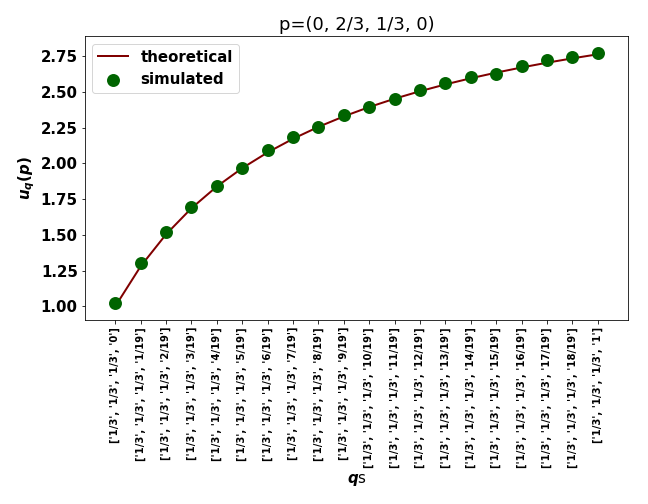
\includegraphics[width=\linewidth]{img/validation_img_two.png}
    \end{subfigure}
    \begin{subfigure}{0.45\textwidth}
        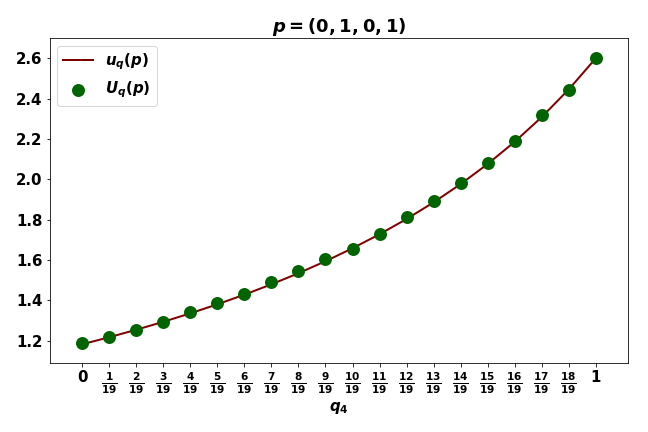
\includegraphics[width=\linewidth]{img/validation_img_three.png}
    \end{subfigure}
\end{center}
\caption{Differences between simulated and analytical results for
\(q = (\frac{1}{3}, \frac{1}{3}, \frac{1}{3}, q_4)\).}
\label{fig:analytical_simulated}
\end{figure}

Moreover Theorem~\ref{theorem:quadratic_form_u} can be expanded to multi opponent
interactions. The IPD is commonly studied in tournaments where a strategy interacts
with a number of opponents. There the payoff of a player is given by the average
payoffs the player achieved. More specifically the expected utility of a memory one strategy
against a \(N\) number of opponents is given by Theorem~\ref{theorem:tournament_utility}.

\begin{theorem}\label{theorem:tournament_utility}
    The expected utility of a memory one strategy \(p\in\mathbb{R}_{[0,1]}^4\)
    against a group of opponents \(q^{(1)}, q^{(2)}, \dots, q^{(N)}\), denoted
    as \(\frac{1}{N} \sum\limits_{i=1} ^ {N} {u_q}^{(i)} (p)\) is given by:

    \begin{equation}\label{eq:tournament_utility}
        \frac{1}{N} \sum\limits_{i=1} ^ {N} {u_q}^{(i)} (p) = \frac{1}{N}
        \frac{\sum\limits_{i=1} ^ {N} (\frac{1}{2} pQ^{(i)} p^T + c^{(i)} p + a^ {(i)})
        \prod\limits_{\tiny\begin{array}{l} j=1 \\ j \neq i \end{array}} ^ 
        N (\frac{1}{2} p\bar{Q}^{(i)} p^T + \bar{c}^{(i)} p + \bar{a}^ {(i)})}
        {\prod\limits_{i=1} ^ N (\frac{1}{2} p\bar{Q}^{(i)} p^T + \bar{c}^{(i)} p + \bar{a}^ {(i)})}.
    \end{equation}

\end{theorem}

To validate the formulation of Theorem~\ref{theorem:tournament_utility} we calculate
the simulated and the theoretical payoffs of several memory one strategies against
a set of 10 opponents. The opponents used are the memory one strategies for the tournament
conducted in~\cite{Stewart2012}. The names and a small explanation of the strategic rules are
given by Table~\ref{table:list_stewart_plotkin}, Appendix~\ref{appendix:tables}.
The values of \(\frac{1}{10} \sum\limits_{i=1} ^ {10} u_{q ^{(i)}} (p)\) and
\(\frac{1}{10} \sum\limits_{i=1} ^ {10} U_{q ^{(i)}} (p)\) match (Table~\ref{table:list_stewart_plotkin}),
thus we conclude that the formulation of Theorem~\ref{theorem:tournament_utility} is correct.

\begin{table}[htbp]
    \begin{center}
    \input{tex/stewart_results.txt}
    \end{center}
    \caption{Results of memory one strategies against the strategies in Table~\ref{table:list_stewart_plotkin}.}
    \label{table:list_stewart_plotkin}
\end{table}

The analytical formulation of Theorem~\ref{theorem:tournament_utility} will be
used in the following sections to explore the best response to memory one
strategies.

\section{Best responses to memory one players}\label{section:best_response_mem_one}

In the introduction a question was raised: which memory one strategy is the \textbf{best response}
to a group of memory one strategies? This will be considered as an optimisation problem,
where a memory one strategy \(p\) wants to optimise it's average utility \( \frac{1}{N} \sum u_{q ^{(i)}} (p)\)
against a set opponents \(\{q^{(1)}, q^{(2)}, \dots, q^{(N)} \}\). 

The decision variable is the vector \(p\) and the solitary constraint is that \(p \in \R^4_{[0, 1]} \).
The optimisation problem is given by~(\ref{eq:mo_tournament_optimisation}). Note that
we will considering the sum and not the average utility as their optimisation corresponds
to the same thing.

\begin{equation}\label{eq:mo_tournament_optimisation}
    \begin{aligned}
    \max_p: & \ \sum_{i=1} ^ {N} {u_q}^{(i)} (p) 
    \\
    \text{such that}: & \ p \in \R_{[0, 1]} 
    \end{aligned}
\end{equation}

This work is concerned with an optimisation problem of a ratio of quadratic forms.
It can be verified empirically for the case of a single opponent that there exist at
least one point for which the definition of concavity does not hold.

There is some work on the optimisation on non concave ratios of of quadratic forms
\cite{Beck2009, Hongyan2014}. In these both the numerator and the denominator
of the fractional problem were concave which is not true for our case. 
These results are established in Theorem~\ref{theorem:concavity}.

\begin{theorem}\label{theorem:concavity}
    The utility of a player \(p\) against an opponent \(q\), \(u_q (p)\) given by
    (\ref{eq:optimisation_quadratic}), is not concave. Furthermore neither the
    numeration or the denominator of (\ref{eq:optimisation_quadratic}), are concave.
\end{theorem}

\begin{proof}
    A function \(f(x)\) is said to be concave on an interval \([a, b]\) if, for any
    points \(x_1\) and \(x_2 \in [a, b]\), the function \(-f(x)\) is convex on that
    interval.

    A function \(f(x)\) is convex on an interval \([a, b]\) if for any two
    points \(x_1\) and \(x_2\) in \([a, b]\) and any \(\lambda\) where \(0 < \lambda < 1\),

    \begin{equation}\label{def:convex}
    f (\lambda x_1 + (1 - \lambda )x_2 ) \leq \lambda f (x_1 ) + (1 - \lambda )f (x_2 ).
    \end{equation}

    Using numerical trials we have shown that there exists at least on point for which
    (\ref{eq:optimisation_quadratic}) is not concave. Let \(f\) be
    \(u_{(\frac{1}{3}, \frac{1}{3}, \frac{1}{3}, \frac{1}{3})}\) it can shown that
    for \(x_1 = (\frac{1}{4}, \frac{1}{2}, \frac{1}{5} , \frac{1}{2}), 
    x_2 = (\frac{8}{10}, \frac{1}{2}, \frac{9}{10} , \frac{7}{10})\) and \(\lambda=\frac{1}{10}\)
    condition (\ref{def:convex}) does not hold as:

    \[1.49 \geq 1.48\]

    Moreover, any potential benefits from the structure of the numerator and the denominator
    are also investigated. In~\cite{Anton2014} it is stated that a quadratic form will
    be concave if and only if it's symmetric matrix is negative semi definite.
    A matrix\(A\) is semi-negative definite if:

    \begin{equation}\label{def:semi_negative}
    |A|_i \leq 0 \text{ for } i \text{ is odd and } |A|_i \geq 0  \text{ for } i
    \text{ is even.}
    \end{equation}

    For both \(Q\) and \(\bar{Q}\) it is exhibited that for \(i=2\) (odd):

    \[|Q|_2 = - \left(q_{1} - q_{3}\right)^{2} \left(q_{2} - 5 q_{4} - 1\right)^{2},\]
    \[|\bar{Q}|_2 =- \left(q_{1} - q_{3}\right)^{2} \left(q_{2} - q_{4} - 1\right)^{2}\]

    both determinants are negative, thus the concavity condition (\ref{def:semi_negative})
    fails for both quadratic forms.
\end{proof}

The non concavity of \(u(p)\) indicates multiple local optimal points. Thus we
are not searching a single optimal point but a set of candidate optimal points.
The aim is to introduce a compact way of constructing the candidate set. Once
the set is defined the point that maximises (\ref{eq:tournament_utility}) corresponds to the best
response strategy, thus any search over an infinitely sized continuous set can instead
be replaced with a discrete set.

The problem considered is a bounded because \(p \in \R^4_{[0, 1]}\). It is known that
the candidate solutions will exist either at the boundaries
of the feasible solution space, or within that space. The method of Lagrange
Multipliers~\cite{bertsekas2014} and Karush-Kuhn-Tucker conditions~\cite{Giorgi2016}
are based on this. The Karush-Kuhn-Tucker conditions are used here because the constraints
are inequalities.

Note that the best response can not be captured by optimising against the mean
opponent.

\begin{equation}\label{eq:tournament_hypothesis}
    \frac{1}{N} \sum_{i=1} ^ {N} {u_q}^{(i)} (p) \neq
      u_{\frac {1}{N} \sum\limits_{i=1} ^ N q^{(i)}}(p).
\end{equation}

A number of numerical experiments have been performed for cases where \(p=(p, p, p, p)\)
and \(p= (p_1, p_2, p_1, p_2)\). This was done in order to compare the right hand
side of equation~(\ref{eq:tournament_hypothesis}) to the left. The fact that
equation~(\ref{eq:tournament_hypothesis}) holds is evident by Figure~\ref{fig:hypothesis}.

\begin{figure}[!htbp]
    \begin{center}
        \begin{subfigure}{0.44\textwidth}
            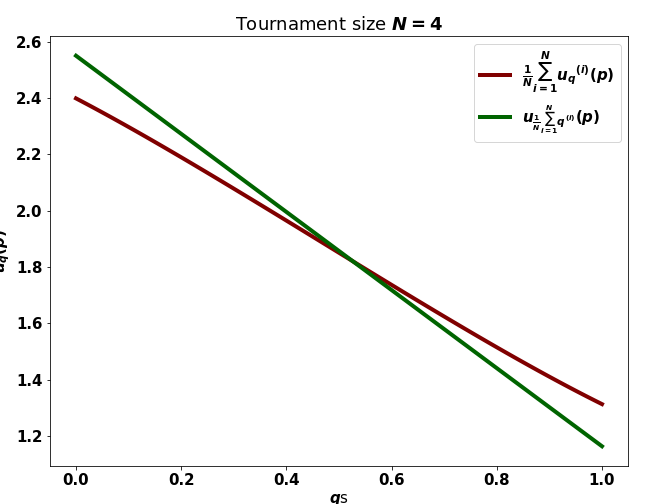
\includegraphics[width=\linewidth]{img/mean_vs_average.png}
        \end{subfigure}
        \begin{subfigure}{0.45\textwidth}
            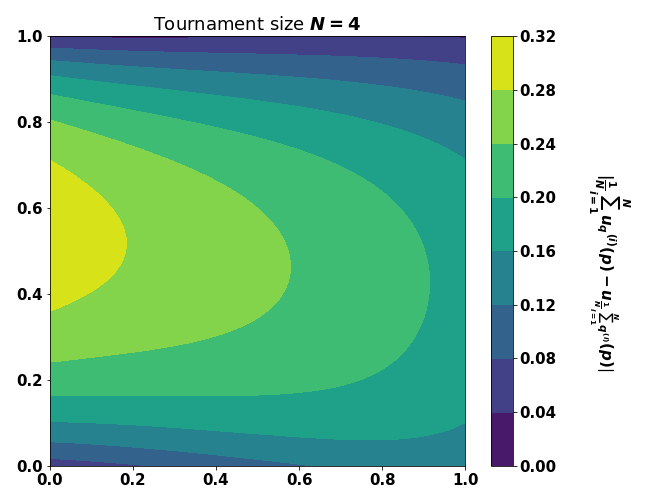
\includegraphics[width=\linewidth]{img/mean_vs_average_two.png}
        \end{subfigure}
    \end{center}
    \caption{An example confirming equation~(\ref{eq:tournament_hypothesis}) for \(p=(p, p, p, p)\)
    and \(p= (p_1, p_2, p_1, p_2)\).}
    \label{fig:hypothesis}
\end{figure}

The above discussion leads to Lemma~\ref{lemma:memone_group_best_response} which
presents the best memory one response to a group of opponents.

\begin{lemma}\label{lemma:memone_group_best_response}
    The optimal behaviour of a memory one strategy player \(p^* \in \R_{[0, 1]} ^ 4\)
    against a set of \(N\) opponents \(\{q^{(1)}, q^{(2)}, \dots, q^{(N)} \}\)
    for \(q^{(i)} \in \R_{[0, 1]} ^ 4\) is established by:
    
    \[p^* = \textnormal{argmax}(\sum\limits_{i=1} ^ N  u_q(p)), \ p \in S_q,\]
    
    where the set \(S_q\) is defined as 
    
    \[S_q = \{0, \bar{p_i}, 1 \}^4 \text{ for } i \in \R,\]
    
    where \(\bar{p_i}\) satisfies one of the following cases:

    \begin{equation}\label{eq:cases_mem_one}\resizebox{.7\hsize}{!}{$
        \left\{\begin{array}{lr}
        \frac{d\sum u}{dp} (p^*) = 0, & \text{for } p^* \in \{\bar{p}_i\} ^ 4, \\
        \frac{d\sum u}{dp_j} (p^*) = 0, & \text{for } p^* \in \{0, \bar{p}_i, 1\} ^ 4
        \text{ where } p_j ^ * \in \{\bar{p}_i\} \text{ for } j \in [1, 4].\\
        \end{array}\right.$}
    \end{equation}

    Equations~(\ref{eq:cases_mem_one}) corresponds to the partial derivatives of the
    utility. For the partial derivatives to be zero, the numerator must fall
    to zero. The numerator of the partial derivatives is given by,

    \begin{equation}\label{eq:group_derivative_numerator_condition}
    (\sum\limits_{i=1} ^ {N} Q_{N}^{(i)'} \prod_{\substack{j=1 \\ j \neq i}} ^ N Q_{D}^{(i)}
     + \sum\limits_{i=1} ^ {N} Q_{D}^{(i)'} \sum_{\substack{j=1 \\ j \neq i}} ^ {N} Q_{N}^{(i)}
    \prod_{\substack{j=1 \\ j \neq \{i, j\}}} ^ N Q_{D}^{(i)}) \times
    \prod\limits_{i=1} ^ N Q_{D}^{(i)} - (\sum\limits_{i=1} ^ {N} Q_{D}^{(i)'}
    \prod_{\substack{j=1 \\ j \neq i}} ^ N Q_{D}^{(i)}) \times 
    (\sum\limits_{i=1} ^ {N} Q_{N}^{(i)} \prod_{\substack{j=1 \\ j \neq i}} ^ N Q_{D}^{(i)})
    \end{equation}

    and the denominator can not nullified, thus:

    \begin{equation}\label{eq:group_derivative_denominator_condition}
        \prod\limits_{i=1} ^ N Q_{D}^{(i)} \neq 0
    \end{equation}

    where,

    \begin{align*}
        Q_{N}^{(i) } & = \frac{1}{2} pQ^{(i)} p^T + c^{(i)} p + a^ {(i)}, \\
        Q_{N}^{(i)'} & =  pQ^{(i)} + c^{(i)}, \\
        Q_{D}^{(i) } & = \frac{1}{2} p\bar{Q}^{(i)} p^T + \bar{c}^{(i)} p + \bar{a}^ {(i)}, \\
        Q_{D}^{(i)'} & =  p\bar{Q}^{(i)} + \bar{c}^{(i)}. \\
    \end{align*}
\end{lemma}

\begin{proof} The best response of a memory one strategy against a group of memory
    one strategies can captured by a candidate set of behaviours. This candidate
    set is constructed by considering behaviours where any or all of \(p_1, p_2, p_3, p_4\)
    are \(\in \{0, 1\}\) and the rest or all of \(p_1, p_2, p_3, p_4\) are given by
    roots of the partial derivatives.

    Note that for \(p_i \in \{0, 1\}\) we consider the roots of the partial derivatives
    for \(p_j \neq p_i\) for \(i,j \in [1, 4]\).

    The derivatives, \(\frac{d\sum u}{dp}\), are given by,

    {\scriptsize
    \begin{align}\label{eq:mo_tournament_derivative}
        \frac{d}{dp} \sum\limits_{i=1} ^ {N} {u_q}^{(i)} (p) & = \nonumber \\
        & =\frac{
        (\sum\limits_{i=1} ^ {N} Q_{N}^{(i)'} \prod_{\substack{j=1 \\ j \neq i}} ^ N Q_{D}^{(i)}
        + \sum\limits_{i=1} ^ {N} Q_{D}^{(i)'} \sum_{\substack{j=1 \\ j \neq i}} ^ {N} Q_{N}^{(i)}
       \prod_{\substack{j=1 \\ j \neq \{i, j\}}} ^ N Q_{D}^{(i)}) \times
       \prod\limits_{i=1} ^ N Q_{D}^{(i)} - (\sum\limits_{i=1} ^ {N} Q_{D}^{(i)'}
       \prod_{\substack{j=1 \\ j \neq i}} ^ N Q_{D}^{(i)}) \times 
       (\sum\limits_{i=1} ^ {N} Q_{N}^{(i)} \prod_{\substack{j=1 \\ j \neq i}} ^ N Q_{D}^{(i)})}
        {(\prod\limits_{i=1} ^ N Q_{D}^{(i)})^{2}}
    \end{align}
    }

    For equation~\ref{eq:mo_tournament_derivative} to be zero, the numerator must fall
    to zero and the denominator can not nullified.

    One the candidate set is constructed each point is evaluated using equation
    (\ref{eq:tournament_utility}). The point with the maximum utility is selected.
\end{proof}

A special case of Lemma~\ref{lemma:memone_group_best_response} is for \(N=1\),
thus when a strategy plays against a single opponent. In this case the formulation
of Theorem~\ref{theorem:quadratic_form_u} is used and the best response is captured
by Lemma~\ref{lemma:memone_best_response}.

\begin{lemma}\label{lemma:memone_best_response}
    The optimal behaviour of a memory one strategy player \(p^* \in \R_{[0, 1]} ^ 4\)
    against a given opponent \(q \in \R_{[0, 1]} ^ 4\) is given by:
    
    \[p^* = \textnormal{argmax}(u_q(p)), \ p \in S_q,\]
    
    where the set \(S_q\) is defined as 
    
    \[S_q = \{0, \bar{p}_i, 1 \}^4 \text{ for } i \in \R,\]
    
    where any \(\bar{p}\) satisfy condition (\ref{eq:cases_mem_one}). Note that now
    the numerators of the partial derivatives, (\ref{eq:group_derivative_numerator_condition}),
    are given by
    
    {\small
    \begin{equation}\label{eq:derivative_numerator_condition}
        (pQ + c) ( \frac{1}{2} p  \bar{Q}  p^T + \bar{c}  p + \bar{a}) 
        - (p\bar{Q} + \bar{c})( \frac{1}{2} p  Q  p^T + c p + a)
    \end{equation}}

    and (\ref{eq:group_derivative_denominator_condition}) is re-written as:

    {\small
    \begin{equation}\label{eq:derivative_denominator_condition}
        \frac{1}{2} p  \bar{Q}  p^T + \bar{c}  p + \bar{a} \neq 0
    \end{equation}}
\end{lemma}

Equations (\ref{eq:group_derivative_numerator_condition}) and (\ref{eq:derivative_numerator_condition})
are systems of maximum \(4\) polynomials and the degree of the polynomials is gradually increasing
every time an extra opponent is taken into account. Solving system of polynomials corresponds
to the calculation of a resultant and for large systems these quickly become intractable.
Because of that no further analytical consideration is given to problems described
here.

Lemma~\ref{lemma:memone_group_best_response} and Theorem~\ref{theorem:tournament_utility}
will now be used to give a list of particular best response results.

\subsection{Reactive Strategies}\label{section:reactive_analytical}

The first constrained case considered here is that of the reactive strategies.
Reactive strategies are a set of memory one strategies where they only take into
account the opponent's previous moves. As described in Section~\ref{section:introduction}
Tit for Tat is a reactive strategy. The optimisation problem of (\ref{eq:mo_tournament_optimisation})
now has an extra constraint and is re written as,

\begin{equation}\label{eq:reactive_tournament_optimisation}
\begin{aligned}
\max_p: & \ \sum_{i=1} ^ N u_q(p)
\\
\text{such that}: & \ p_1 = p_3 \text{ and } p_2 = p_4\\
    & \ p_1, p_2 \in \R_{[0, 1]}.
\end{aligned}
\end{equation}

Reactive strategies allow us to study \(u_p\) as a function of two variables
\(p_1, p_2\) and the best reactive response against a group of opponents is captured by Lemma
\ref{lemma:reactive_group_best_response}.

\begin{lemma}\label{lemma:reactive_group_best_response}
    The optimal behaviour of a reactive player \(p^* \in \R_{[0, 1]} ^ 2\) against a set
    of \(N\) opponents \(\{q^{(1)}, q^{(2)}, \dots, q^{(N)} \}\) for \(q^{(i)} \in 
    \R_{[0, 1]} ^ 4\) is given by:

    \[p^* = \textnormal{argmax}(\sum\limits_{i=1} ^ N  u_q(p)), \ p \in S_q,\]
    
    where the set \(S_q\) is defined as 
    
    \[S_q = \{0, \bar{p_i}, 1 \} ^ 2 \text{ for } i \in \R,\]
    
    where \(\bar{p_i}\) satisfies one of the following cases:

    \begin{equation}\label{eq:cases_reactive}
        \left\{\begin{array}{lr}
        \frac{\sum u}{dp} (p^*) = 0, & \text{for } p^* \in \{\bar{p}_i\} ^ 4, \\
        \frac{\sum u}{dp_1} (p^*) = 0, & \text{for } p_1^* \in \{\bar{p}_i\}
        \text{ while } p_2 ^ * \in \{0, 1\},\\
        \frac{\sum u}{dp_2} (p^*) = 0, & \text{for } p_2^* \in \{\bar{p}_i\}
        \text{ while } p_1 ^ * \in \{0, 1\}.
        \end{array}\right.
    \end{equation}

    For cases (\ref{eq:cases_reactive}) to be true the numerator of the partial
    derivatives, given by (\ref{eq:group_derivative_numerator_condition}), must equal
    to zero and condition (\ref{eq:group_derivative_denominator_condition}) must hold.
\end{lemma}

Similarly to the memory one approach a special case for \(N=1\), against a single
memory one strategy, is applied to
Lemma~\ref{lemma:reactive_group_best_response}. The best response against a single
opponent is captured by Lemma~\ref{lemma:reactive_best_response}.

\begin{lemma}\label{lemma:reactive_best_response}
    The optimal behaviour of a reactive player \(p^* \in \R_{[0, 1]} ^ 2\) against a given
    opponent \(q \in \R_{[0, 1]} ^ 4\) is given by:
    
    \[p^* = \textnormal{argmax}(u_q(p)), \ p \in S_q,\]
    
    where the set \(S_q\) is defined as 
    
    \[S_q = \{0, \bar{p_i}, 1 \} ^ 2 \text{ for } i \in \R,\]
    
    where \(\bar{p}_i\) satisfies any of (\ref{eq:cases_reactive}). Partial derivatives
    are now given by (\ref{eq:derivative_numerator_condition}) and
    (\ref{eq:derivative_denominator_condition}) must be true.
\end{lemma}

Note that now equation (\ref{eq:group_derivative_numerator_condition}) and (\ref{eq:derivative_numerator_condition})
correspond to systems of maximum 2 polynomials over 2 variables. Each polynomial is equivalent
to a partial derivative over \(p_1\) and \(p_2\). Several methods exist that allow
for the \(2\) polynomial systems to be solved analytically. In this work the results theory
is used to extract the roots from the partial derivatives.

Note that for pairwise interactions the maximum degree
of the polynomials is equal to \(2N\), however the degree increases as opponents
are introduced.

The resultant is a symmetric function of the roots of the polynomials of a system
and it can be expressed as a polynomial in the coefficients of the polynomials.
The resultant will equal zero if and only if the system has at least one common
root. Thus, the resultant becomes very useful in identifying whether common roots exist.

In this work the Sylvester's resultant~\cite{Akritas1991} denoted as (\(R_S\))
is considered. The Sylvester's resultant is used to solve system of a single
variable. However, for a system of two variables we solve over one variable and
the second is kept as a coefficient. Thus we can find the roots of the equations
and that is why the resultant is often refereed to as the eliminator.

In Appendix Algorithm~\ref{algo:reactive} describes the process and based on the
Algorithm several examples are performed. Illustrated by Figure~\ref{fig:reactive_pairwise_results}
are the results of these examples. The results suggest that the best response behaviour
is captured by our algorithm.

\begin{figure}
    \centering
    \begin{subfigure}{0.45\textwidth}
        \centering
        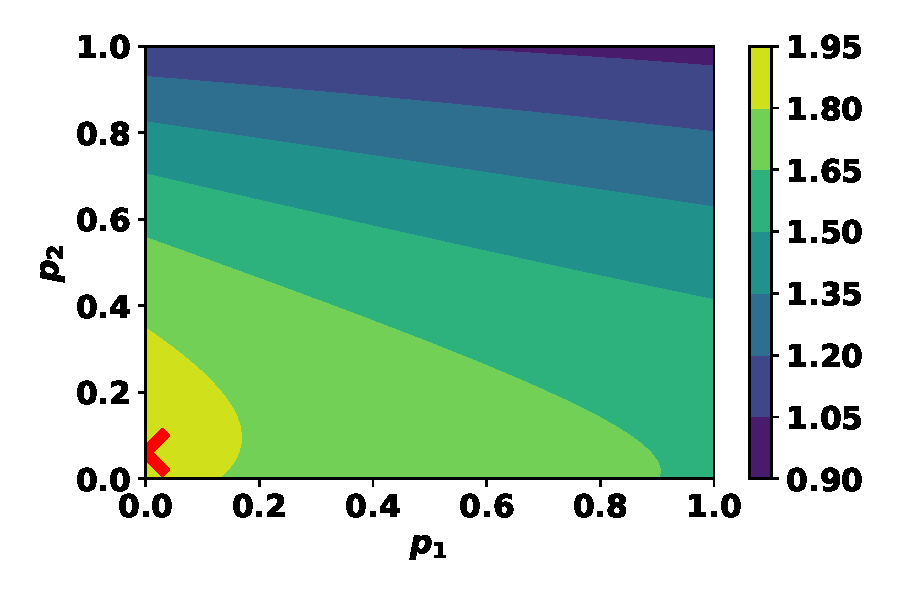
\includegraphics[width=.95\textwidth]{img/reactive_pairwise_one.pdf}
    \end{subfigure}
    \begin{subfigure}{0.45\textwidth}
        \centering
        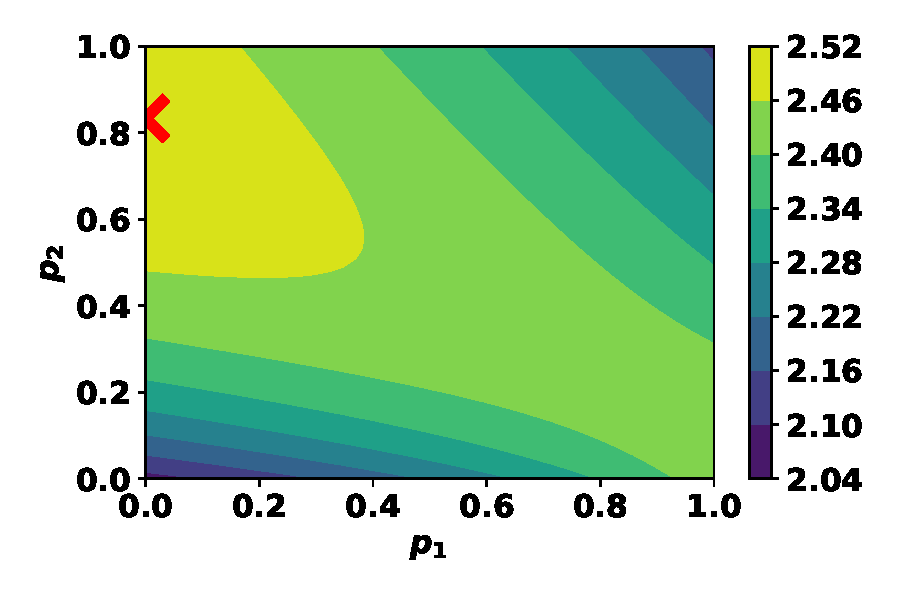
\includegraphics[width=.95\textwidth]{img/reactive_pairwise_two.pdf}
    \end{subfigure}
    \caption{Numerical experiments for Algorithm~\ref{algo:reactive} for \(N=1\).}
    \label{fig:reactive_pairwise_results}
\end{figure}

\subsection{Purely random}\label{section:purely_analytical}

The next constrained problem to be explored is that of the purely random strategies.
Purely random strategies are a set of memory one strategies where the transition
probabilities of each state are the same. The optimisation problem of (\ref{eq:mo_tournament_optimisation})
now has an extra constraint and is re written as,

\begin{equation}\label{eq:random_optimisation}
\begin{aligned}
\max_p: & \ \frac{1}{N} \sum_{i=1} ^ {N} {u_q}^{(i)} (p) 
\\
\text{such that}: & p_1 = p_2 = p_3 = p_4 = p \\
                  & p \in \R_{[0, 1]} \\
\end{aligned}
\end{equation}

and the exact optimal behaviour of purely random strategies is described in
Lemma~\ref{lemma:purely_optimisation}.

\begin{lemma}
    \label{lemma:purely_optimisation}
    The optimal behaviour of a \textbf{purely random} player \(p ^ * \in \R_{[0, 1]}\)
    in an \(N-\)memory one player tournament, \(\{q_{(1)}, q_{(2)} \dots,q_{(N)} \}
    \) for \(q_{(i)} \in \R_{[0, 1]} ^ 4\) is given by:
    
    \[p^* = \textnormal{argmax}(\sum_{i=1} ^ {N} {u_q}^{(i)} (p) ), \ p \in S_{q(i)},\]
    
    where the set \(S_{q}\) is defined as:
    
    \[S_{q} = \{0, \lambda_i, 1\},\text{ for } i \in [1, 2N]\]

    where \(\lambda_i\) are the eigenvalues of the companion matrix corresponding
    to the numerator of \[\frac{d}{dp} \sum_{i=1} ^ {N} {u_q}^{(i)} (p)\]

    for which
    \[\frac{d}{dp} \sum_{i=1} ^ {N} {u_q}^{(i)} (\lambda_j) = 0,\text{ for } j \in [1, 2N].\]
\end{lemma}

\begin{proof}
    The best behaviour of a purely random strategy against a set of opponents is
    captured by a set of potential best behaviours. For constructing this a set
    a similar as the ones described in previous sections is used.

    It is know that \(p ^ *\) will either be \(\in \{0, 1\}\) or \(p ^ *\) will because
    given by the roots of \(\frac{d}{dp} \sum\limits_{i=1} ^ {N} {u_q}^{(i)}(p)\).
    The roots of  \(\frac{d}{dp} \sum\limits_{i=1} ^ {N} {u_q}^{(i)} (p)\) are the roots 
    only of the numerator, as the denominator can not be nullified.

    Studying equation (\ref{eq:optimisation_quadratic}) as a function of a single variable
    \(p\) it can be verified that the degree of the numerator is equal to\(2N\).
    Thus, the size of roots of the numerator is equal to \(2N\).

    The roots on the polynomial in this work will be calculated using a companion
    matrix method~\cite{Edelman1995}. This method allows the roots of the polynomial to
    be computed by calculating the eigenvalues of the corresponding companion
    matrix.

    The eigenvalues and the bounds compose the candidate set of solutions. The
    best response of a purely random player corresponds to the point that maximises
    (\ref{eq:optimisation_quadratic}).
\end{proof}

Lemma~\ref{lemma:purely_optimisation} can be further expanded to the case where \(N=1\).
Algorithm~\ref{algo:purely} describes the process of best purely random responses and it is
used for a number of empirical trials.
The results of these trials are illustrated in Figures~\ref{fig:purely_random_pairwise_results}
and \ref{fig:purely_random_tournament_results}. Figure~\ref{fig:purely_random_pairwise_results}
demonstrates Lemma~\ref{lemma:purely_optimisation} for \(N=1\) and
Figure~\ref{fig:purely_random_tournament_results} cases were \(N>1\).
It is evident that the optimal behaviour has been captured by our search algorithm.

\begin{figure}
    \centering
    \begin{subfigure}{0.45\textwidth}
        \centering
        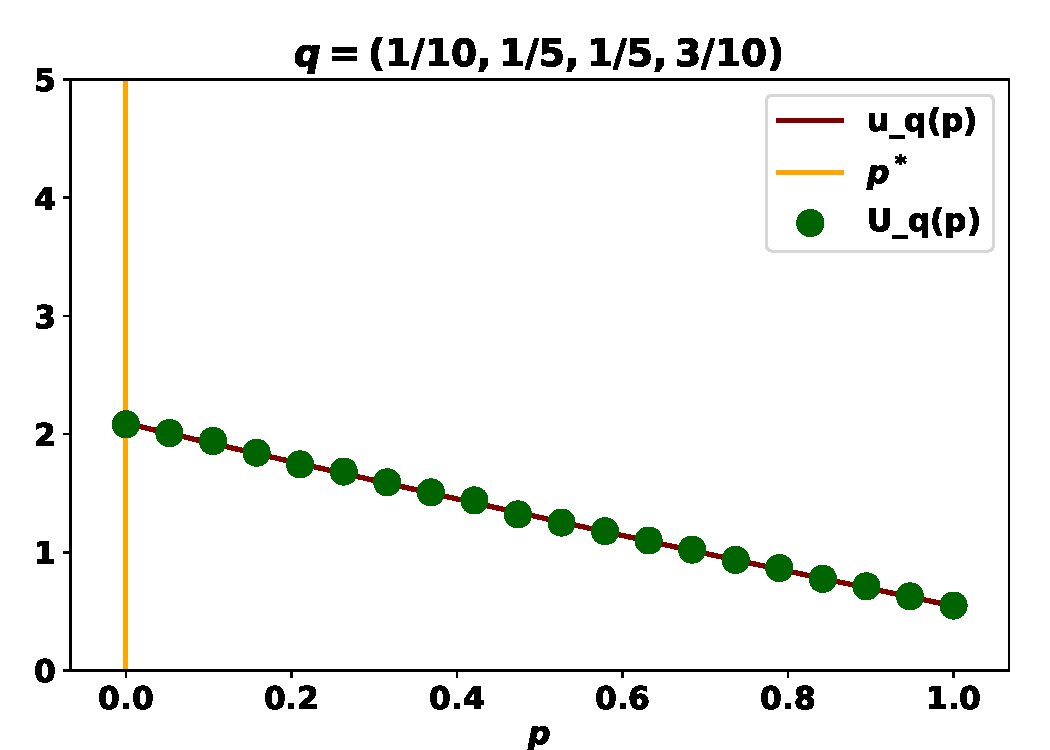
\includegraphics[width=.95\textwidth]{img/purely_random_match_one.pdf}
    \end{subfigure}
    \begin{subfigure}{0.45\textwidth}
        \centering
        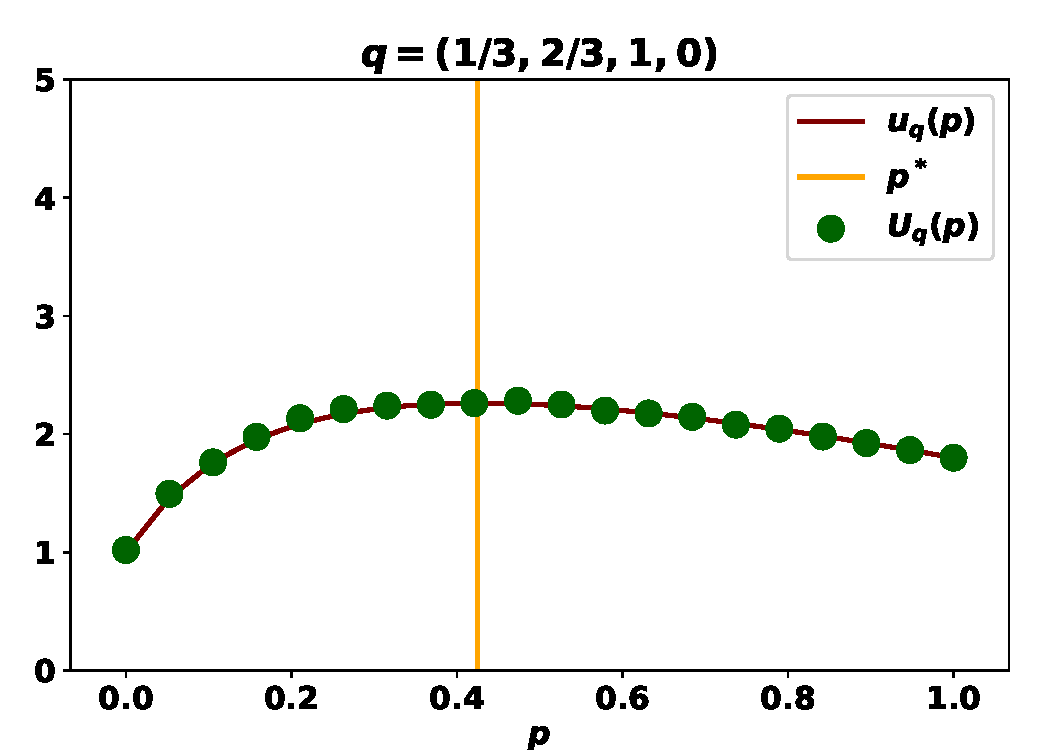
\includegraphics[width=.95\textwidth]{img/purely_random_match_two.pdf}
    \end{subfigure}
    \caption{Numerical experiments for Algorithm~\ref{algo:purely} for \(N=1\).}
    \label{fig:purely_random_pairwise_results}
\end{figure}

\begin{figure}
    \centering
    \begin{subfigure}{0.45\textwidth}
        \centering
        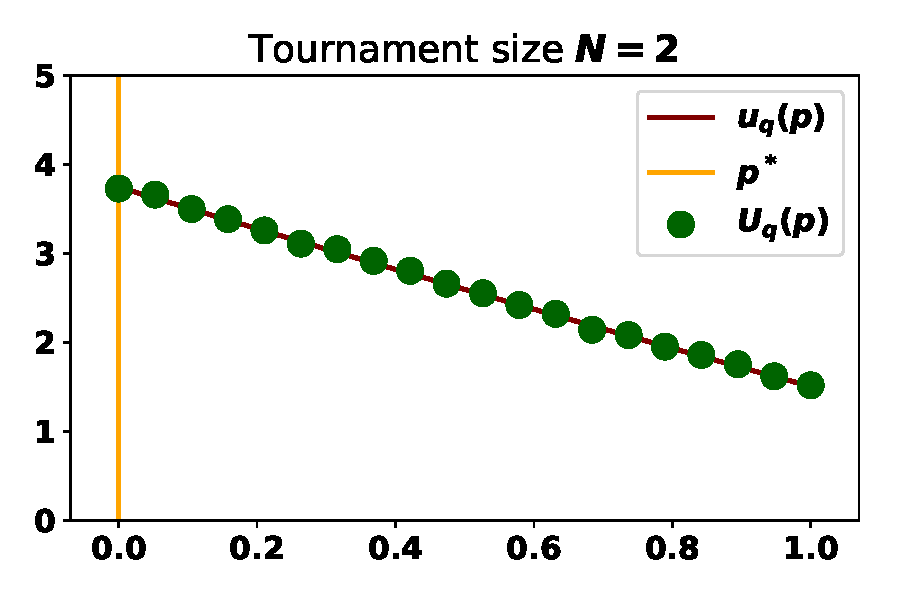
\includegraphics[width=.95\textwidth]{img/purely_random_tournament_one.pdf}
    \end{subfigure}
    \begin{subfigure}{0.45\textwidth}
        \centering
        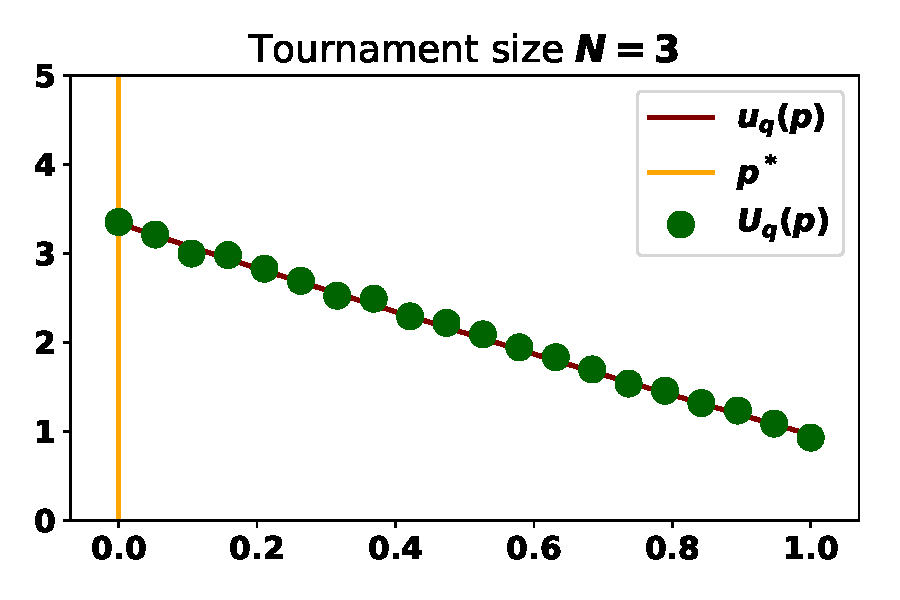
\includegraphics[width=.95\textwidth]{img/purely_random_tournament_two.pdf}
    \end{subfigure}
    \caption{Numerical experiments for Algorithm~\ref{algo:purely} for \(N>1\).}
    \label{fig:purely_random_tournament_results}
\end{figure}

Furthermore, for the case of the purely random players two more theoretical results
are discussed. These are the cases where the opponent has manage to make a random
player indifferent and the case where a purely random player is better of playing
a pure strategy.

There is importance in both results. Initially, being indifferent refers to our
actions no having any effects on the match. Thus there is not optimal behaviour
for player \(p\).

Secondly, by a pure strategy we are referring to the \(p=0\) and \(p=1\).
In this case it is know that \(p^*\) is \(\in {0, 1}\) without testing the roots
of the derivative. The optimisation problem crumbles to a binary problem.

The results are given equivalently by Lemmas~\ref{lemma:constant} and~\ref{lemma:linear}
and they are respective to the actions of the opponent. Figure~\ref{fig:purely_lemmas}
illustrates examples for both lemmas.

\begin{lemma}\label{lemma:constant}
    A given memory one player, \((q_1, q_2, q_3, q_4)\), makes a \textbf{purely
    random} player, \((p, p, p, p)\), indifferent if and only if, 
    \(-q_1 + q_2 + 2q_3 - 2q_4 = 0 \) and 
    \((q_2 - q_4 - 1)(q_1 - 2q_2 - 5q_3 + 7q_4 + 1) -(q_2 - 5q_4 - 1)(q_1 - q_2 - q_3 + q_4) = 0 \).
\end{lemma}

\begin{lemma}\label{lemma:linear}
    Against a memory one player, \((q_1, q_2, q_3, q_4)\), a \textbf{purely random}
    player would always play a pure strategy if and only if
    \((q_{1}q_{4} - q_{2} q_{3} + q_{3} - q_{4}) (4 q_{1} - 3 q_{2} - 4 q_{3} + 3 
    q_{4} - 1) = 0\).
\end{lemma}

\begin{figure}[!htbp]
    \begin{center}
        \begin{subfigure}{0.45\textwidth}
            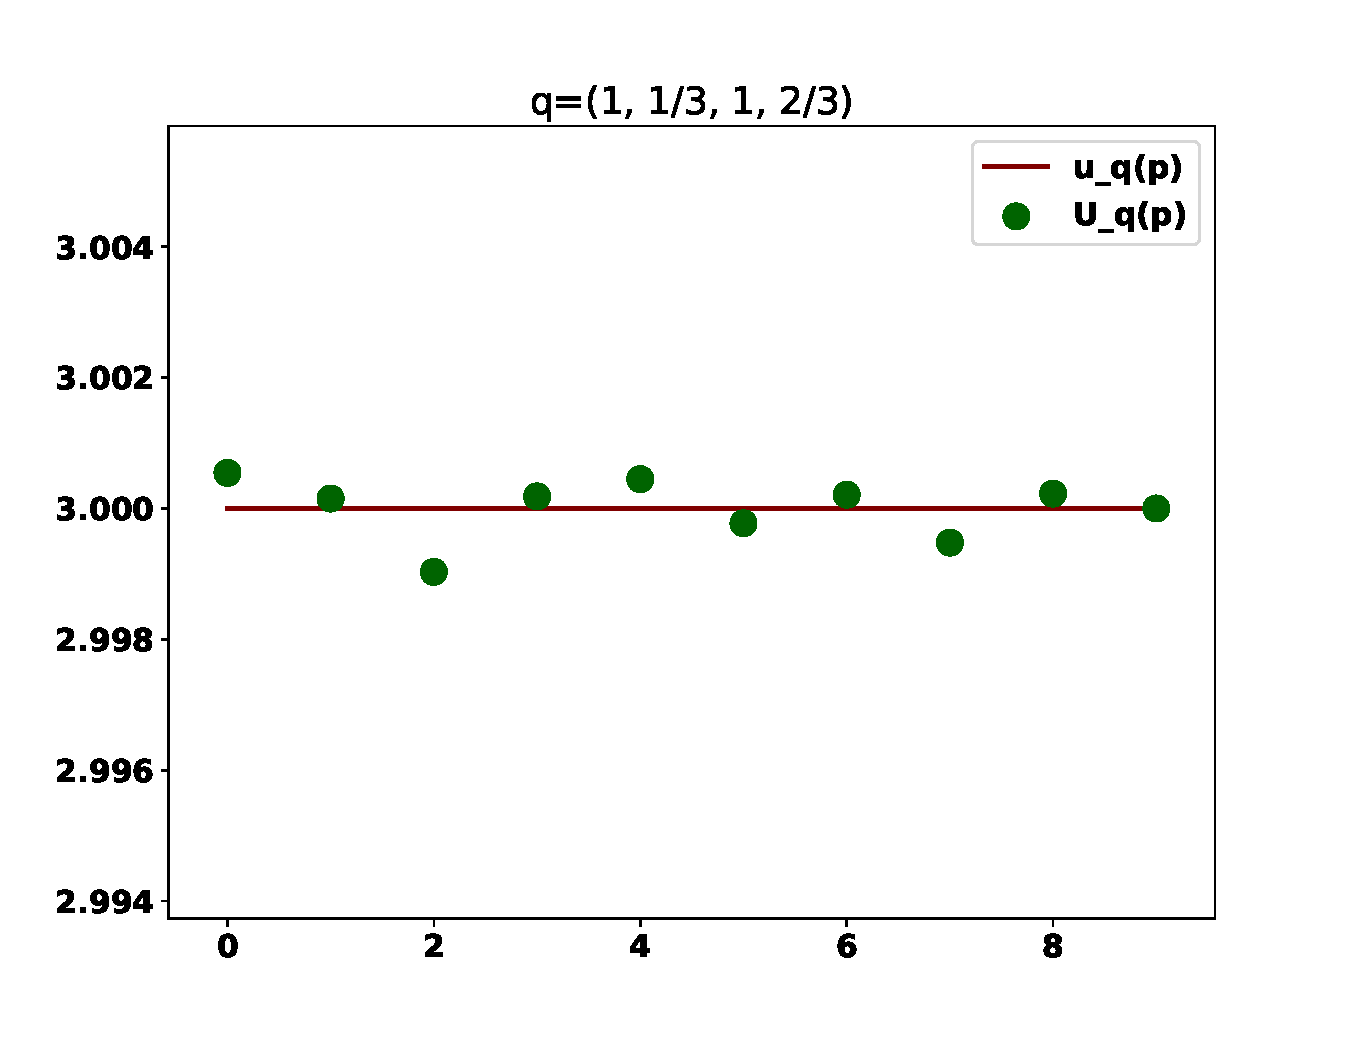
\includegraphics[width=\linewidth]{img/constant}
        \end{subfigure}
        \begin{subfigure}{0.45\textwidth}
            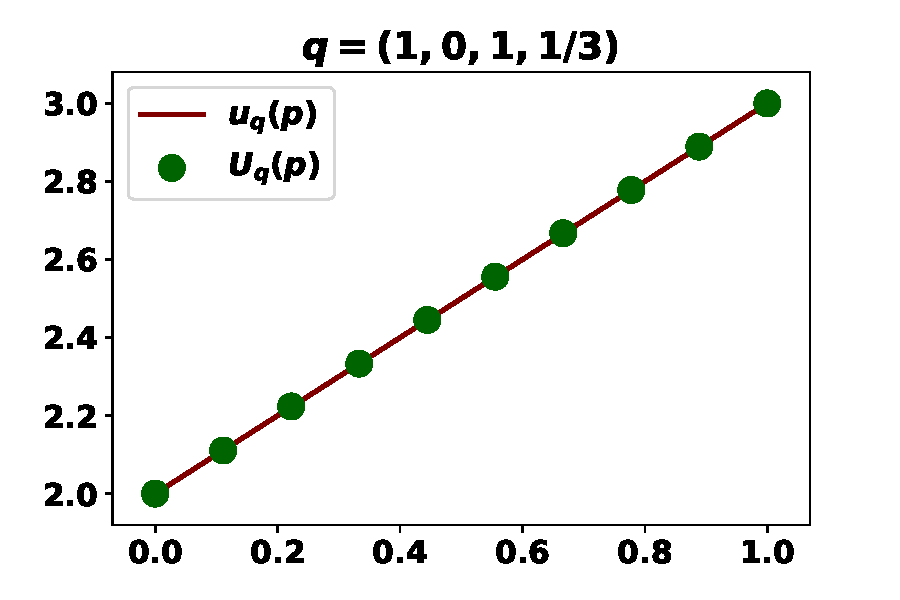
\includegraphics[width=\linewidth]{img/linear}
        \end{subfigure}
    \end{center}
    \caption{Proof of concept for Lemmas~\ref{lemma:constant},~\ref{lemma:linear}.}
    \label{fig:purely_lemmas}
\end{figure}

\section{Stability of defection}

In this section the stability of defection is explored. Defection is
known to be the dominant action in the PD and it can be proven to be the dominant
strategy for the IPD for given environments. Even so, several works have proven
that cooperation emerges in the IPD many studies around the game focus on the
emergence of cooperation. In this manuscript we try to provide a condition for when
defection is the best response in the IPD, thus when it is known that cooperation can
not occur.

This will be done by considering equation~(\ref{eq:mo_tournament_derivative}).
Let equation~(\ref{eq:mo_tournament_derivative}) for \(p = (0, 0, 0, 0)\),

\begin{equation}\label{eq:derivative_of_quadratic_zero}
    \begin{aligned}
     \frac{du}{dp_{| p=(0, 0, 0, 0)}} & = && \frac{c \bar{a} - \bar{c}a}
      {\bar{a}^2} .\\
    \end{aligned}
\end{equation}

The numerator \(\bar{c}a - c\bar{a}\) is given by,

\[\input{tex/defection_matrix.txt}\]

and the denominator \(\bar{a} ^ 2 = (-q_2 + q_4 + 1) ^ 2\), which is always positive. In order
for defection to be the best response the derivative must have a negative
sign at the point \(p = (0, 0, 0, 0)\). That means that the utility is only
decreasing after \(p = (0, 0, 0, 0)\).

Because \(\bar{a} ^ 2\) is always positive the sign of the derivative is given by \(\bar{c}a - c\bar{a}\).
More specifically from equations,

\begin{equation}\label{eq:defection_condition_one}
    \input{tex/defection_condition_one.txt}
\end{equation}
\begin{equation}\label{eq:defection_condition_two}
    \input{tex/defection_condition_two.txt}
\end{equation}

Both signs of the partial derivatives must be negative in order for the overall
function to be decreasing, thus defection being the best response.
The signs of equations (\ref{eq:defection_condition_one}) and (\ref{eq:defection_condition_two})
vary. There are cases that they have the same sign and cases that they do not,
this is shown by numerical example summarized in Table~\ref{table:sign_of_derivative}.

\begin{table}[htbp]
\begin{center}
\begin{tabular}{cllllcc}
    \toprule
    {}& {} & {}& {}& {}&  equation(\ref{eq:defection_condition_one}) &  equation(\ref{eq:defection_condition_two}) \\
    \midrule
1 & \(q_1=\frac{3}{10}\),   & \(q_2=\frac{3}{20}\),  & \(q_3=\frac{13}{20}\), & \(q_4=\frac{7}{100}\)
&  + & + \\
2 & \(q_1=\frac{11}{25}\),  & \(q_2=\frac{3}{10}\),  & \(q_3=\frac{9}{10}\),  & \(q_4=\frac{1}{2}\)
&  - & - \\
3 & \(q_1=\frac{17}{20}\),  & \(q_2=\frac{3}{4}\),   & \(q_3=\frac{2}{5}\),   & \(q_4=\frac{1}{4}\)
&  - & + \\
4 & \(q_1=\frac{13}{88}\),  & \(q_2=\frac{21}{92}\),  & \(q_3=\frac{21}{26}\),  & \(q_4=\frac{20}{67}\)
&  + & - \\
    \bottomrule
\end{tabular}
\end{center}
\caption{Numerical examples of the derivative's sign.}
\label{table:sign_of_derivative}
\end{table}

For a tournament setting we substitute \(p_0\) in equation~(\ref{eq:mo_tournament_derivative}):

\begin{equation}
\sum_{i=1} ^ N (c^{(i)T} \bar{a}^{(i)} - \bar{c}^{(i)T} a^{(i)})
\prod\limits_{\tiny\begin{array}{l} j=1 \\ j \neq i \end{array}} ^ N (\bar{a}^{(i)})^2
\end{equation}

The product term \(\prod\limits_{\tiny\begin{array}{l} j=1 \\ j \neq i \end{array}} ^ N (\bar{a}^{(i)})^2\)
is known to always be positive. However the sign of the sum term 
\(\sum_{i=1} ^ N (c^{(i)T} \bar{a}^{(i)} - \bar{c}^{(i)T} a^{(i)})\) can vary based
on the transition probabilities of the opponents, as discussed above. A condition that
must hold in order for defection to be stable in a tournament is that the sum term
must be negative. The results are summarised by Lemma~\ref{}.

\begin{lemma}
    In a tournament of \(N\) players where \(q^(i) = (q_{1}^(i), q_{2}^(i), q_{3}^(i), q_{4}^(i))\)
    defection is known to be a best response if the transition probabilities of the
    opponents satisfy the condition:

    \begin{equation}
        \sum_{i=1} ^ N (c^{(i)T} \bar{a}^{(i)} - \bar{c}^{(i)T} a^{(i)}) <= 0.
    \end{equation}
\end{lemma}

Moreover lets us consider a constrained version of the problem once again. Lets us
assume that in an pairwise interaction the opponent is a reactive player \(q=(q_1, q_2, q_1, q_2)\).
By substituting \(q_3=q_1\) and \(q_4=q_2\) equations (\ref{eq:defection_condition_one})
and (\ref{eq:defection_condition_two}) are now re written as follow,

\[\left[\begin{matrix}- q_{2} \left(4 q_{1} - 5 q_{2} - 1\right)\\
\left(q_{2} - 1\right) \left(4 q_{1} - 5 q_{2} - 1\right)\end{matrix}\right]\]

The sign of both equations is now based on the same term,\(\left(4 q_{1} - 5 q_{2} - 1\right)\),
which is a term that can have both negative and positive values. This is shown
by Figure~\ref{fig:sign_against_reactive}. Following this the following result is retrieved,

\begin{figure}[htbp]
    \centering
    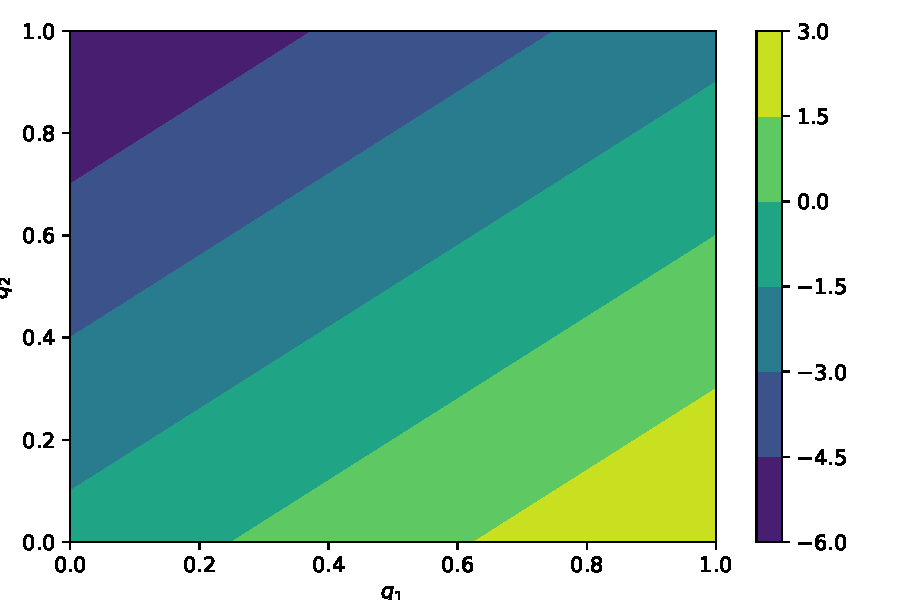
\includegraphics[width=0.45\linewidth]{img/sign_against_reactive.pdf}
      \caption{Sign of \(\left(4 q_{1} - 5 q_{2} - 1\right)\).}
      \label{fig:sign_against_reactive}
  \end{figure}

\begin{lemma}
Defection is the best responses of a memory one player \(p\) against a reactive
player \(q\) if the transition probabilities of the opponent satisfy the
condition:

\begin{equation}
    4 q_{1} - 5 q_{2} - 1 > 0
\end{equation}
\end{lemma}

% \subsection{Memory one strategies}\label{section:mo_numerical}

% As discussed in Section~\ref{section:memory_one_analytical} best responses in memory
% one strategies will be captured using a numerical method. In this
% subsection we discuss the reasons for choosing the specific method and parameters.

% Moreover, a parameter sweep has been performed and here we wil discuss the results.

% Bayesian optimisation is ...

% \section{Limitation of memory}

% The second part of this paper focuses on the limitation of memory size.
% The aim is to show that memory one strategies suffer for multi agent interactions
% whilst they outperform any strategy in pairwise interactions. This is achieved by
% comparing the performance of an optimised short memory one strategies to a trained
% longer memory strategies in tournaments of size 3.

% The complex strategy is trained using the same optimisation algorithm
% as the one described in Section~\ref{section:mo_numerical}, the bayesian
% optimisation. The trained strategy used is a strategy called Gambler.
% Gambler is introduced and discussed in~\cite{Harper2017}.

% \subsection{Gambler}

% Several means of representing strategies have been used over the years for
% IPD strategies. In~\cite{Harper2017} several of those `archetypes' are presented
% and used to train different successful strategies. One of the archetypes firstly
% introduced in that paper is the Gambler.

% Gambler is based on a lookup table and encodes a probability of cooperating
% based on the opponent's first \(n_1\) moves, the opponent's last \(m_1\) moves,
% and the players last \(m_2\) moves.

% Several variants of Gambler have been trained for this work, a summary is given
% by Table. In essence Gambler can represent any generic strategy and that is
% why it has been chosen.

% \begin{table}[htbp]
% \begin{center}
% \begin{tabular}{clllll}
%     \toprule
%     {}&  \(n_1\) & \(m_1\) & \(m_2\)\\
%     \midrule
%     1 & 1 & 1 & 2\\
%     2 & 2 & 2 & 0\\
%     3 & 2 & 2 & 1\\
%     4 & 2 & 2 & 2\\
%     5 & 4 & 4 & 4\\
%     \bottomrule
% \end{tabular}
% \end{center}
% \caption{Variants of Gambler used.}
% \label{table:gambler}
% \end{table}

% \subsection{Procedure}

% For a number of tournaments, where \(N=3\), using the results of Section, we 
% find the optimal best memory one strategy and it's utility. Afterwards, the memory
% on strategy is removed from the tournament and it is replaced with a variant of Gambler
% which is then trained for that environment as well.

% The performance of those two strategies is compared.

% The results of a big parameter sweep are discussed in the following section.

% \subsection{Limitation Results}

% Results, results, results.

% \section{Discussion}

\appendix
\section{Appendix Tables}\label{appendix:tables}

The memory one strategies used in the computer tournament described in~\cite{Stewart2012}
are given by Table~\ref{table:list_stewart_plotkin}.


\begin{table}
        \begin{center}
        \resizebox{.5\textwidth}{!}{\begin{tabular}{clcc}
        \toprule
        {}&  Name & Memory one representation & Reference \\
        \midrule
        1  & Cooperator           & \((1, 1, 1, 1)\) & \cite{Axelrod1981} \\
        2  & Defector             & \((0, 0, 0, 0)\) & \cite{Axelrod1981}\\
        3  & Random               & \((\frac{1}{2}, \frac{1}{2}, \frac{1}{2},
        \frac{1}{2})\) & \cite{Axelrod1981} \\
        4  & Tit for Tat          & \((1, 0, 1, 0)\) & \cite{Axelrod1981}\\
        5  & Grudger              & \((1, 0, 0, 0)\) & \cite{Li2011} \\
        6  & Generous Tit for Tat & \((1, \frac{1}{3}, 1, \frac{1}{3})\) & \cite{Nowak1990}\\
        7  & Win Stay Lose Shift  & \((1, 0, 0, 1)\) & \cite{Nowak1993} \\
        8  & ZDGTFT2              & \((1, \frac{1}{8}, 1, \frac{1}{4})\) &\cite{Stewart2012}\\
        9  & ZDExtort2            & \((\frac{8}{9}, \frac{1}{2}, \frac{1}{3},
        0)\) & \cite{Stewart2012}\\
        10 & Hard Joss            & \((\frac{9}{10}, 0, \frac{9}{10}, 0)\) &
        \cite{Stewart2012} \\
        \bottomrule
    \end{tabular}}
    \caption{List of strategies used in the tournament described in~\cite{Stewart2012}.}
    \label{table:list_stewart_plotkin}
    \end{center}
\end{table}

\section{Appendix Algorithms}

\begin{algorithm}
    \setstretch{1.35}
    \caption{Best response algorithm for reactive strategies}\label{algo:reactive}
    \begin{algorithmic}[1]
    \Procedure{Reactive search}{}
    \State $N \gets \text{number of opponets}$ 
    \State $S_q \gets \{0, 1\} ^ 2$ 
    \State $u' \gets \frac{d\sum\limits_{i=1} ^ {N}u}{d\bar{p}}$ 
    \State $\frac{u_N}{u_D} \gets u'$ 
    \State $S(u_N, p_2) \gets \text{Sylvester's matrix for} p_2. \text{Coefficients are polynomials of } p_1$
    \State $R_S(S) \gets det(S)$
    \State $\text{roots}_{p_1} \gets p_1 \text{ for } det(M)_{p_1} = 0$
    \BState \emph{loop} $\text{root in roots}_{p_1}$:
    \State $\text{ system}(p_2) \gets u_N (root)$
    \State $\text{root}_{p_2} \cup {p_2} \text{ for } \text{system}(p_2) = 0$
    \If {$u_D((\text{root}, \text{root}_{p_2})) \neq 0$}
    \State $S_q \cup \{(\text{root}, \text{root}_{p_2})\}$
    \EndIf
    \State \textbf{goto} \emph{loop}.
    \State \textbf{close};
    \State $p^* \gets \text{argmax}(\sum\limits_{i=1} ^ {N} u_{q^{(i)}} (p)), p \in S_q$.
    \EndProcedure
    \end{algorithmic}
\end{algorithm}

\begin{algorithm}
    \setstretch{1.35}
    \caption{Best response algorithm for purely random strategies}\label{algo:purely}
    \begin{algorithmic}[1]
    \Procedure{Purely random search}{}
    \State $N \gets \text{number of opponets}$ 
    \State $S_q \gets \{0, 1\}$ 
    \State $u' \gets \frac{d\sum\limits_{i=1} ^ {N}u}{d\bar{p}}$ 
    \State $\frac{u_N}{u_D} \gets u'$ 
    \State $C(u_N) \gets \text{companion matrix of } u_N$
    \BState \emph{loop} $i=1 \text{ to } 2N$:
    \State $\lambda_i \gets \text{eigenvalue of } C(u_N)$
    \If {$u_D(\lambda_i) \neq 0$}
    \State $S_q \cup \lambda_i $.
    \EndIf
    \State \textbf{goto} \emph{loop}.
    \State \textbf{close};
    \State $p^* \gets \text{argmax}(\sum\limits_{i=1} ^ {N} u_{q^{(i)}} (p)), p \in S_q $.
    \EndProcedure
    \end{algorithmic}
\end{algorithm}

% Bibliography
\bibliographystyle{plain}
\bibliography{bibliography.bib}

\end{document}

